\section{Research Goals}

\begin{figure}
	\centering
	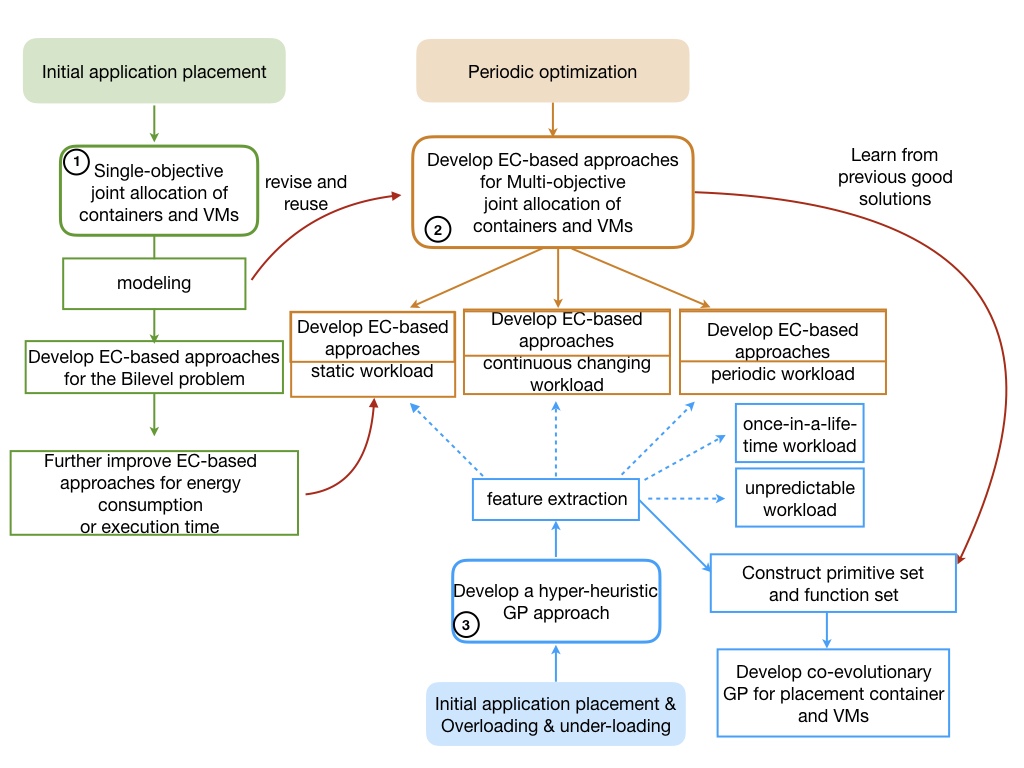
\includegraphics[width=\textwidth]{pics/thesisPlan.jpeg}
	\caption{Relationship between objectives}
	\label{fig:objectives}
\end{figure}

\bx{The overall goal for this thesis is to improve energy efficiency of a container-based Cloud data center with new models and algorithms in three resource management processes:} application initial placement, periodic optimization, and dynamic placement. The specific research objectives of this work can be itemized as follows.
% In this thesis, we aims at providing a series of approaches to continuously optimize the a joint allocation of VMs and containers that considers three consolidation scenarios: Initialization, global consolidation, Dynamic consolidation. In addition, the static allocation normally involves with large amount of variables which is particular difficult to optimize. We are also going to propose a method to solve this problem.  These approaches combine element of AI planning, to ensure the objectives and constraint fulfillment, and of Evolutionary Computation, to evolve a population of near-optimal solutions. The research aims at determining a flexible way in creation of solutions to solve server consolidation problems. As discussed in the previous section, the research goal can be achieved in the following objectives and sub-objectives.

\subsection{Objective One: Develop EC-based approaches for the single objective joint allocation of containers and VMs}
\label{sec:obj1}

\bx{The goal is to reduce the energy consumption in application initial placement considering container-based cloud data center.} To achieve this goal, inevitably, the first step is to propose a new model for container-based placement problem which considers the problem as a bilevel optimization problem. Then, we will explore evolutionary based approaches to solve the problem. The research goal leads to three objectives as follows.
% \textcolor{Maroon}{Currently, most research on container consolidation do not consider the two-level of allocation problem.} Unlike previous VM-based service consolidation, 
% most research focus on VM-based server consolidation technique. They often modeled the VM allocation problem as a vector bin-packing problem \cite{Zhang:2016cx}. 
% Container adds an extra layer of abstraction on top of VM. The placement problem has become a two-step procedure, in the first step, containers are packed into VMs and then VMs are consolidated into physical machines. These two steps are inter-related to each other. Previous research \cite{Piraghaj:2015uf} solve this problem in separated steps where the first step allocates containers to VMs and the second step allocates VMs to PMs with simple bin-packing heuristics. According to Mann's \cite{Mann:2016hx} observation, these two allocations should be conducted simultaneously to reach a near-optima solution, which essentially minimizes the energy consumption.

\begin{enumerate}
	\item Develop a new model to capture the relationship between containers allocation and energy consumption in container-based cloud data center.
	% \textcolor{Maroon}{This problem can be considered as a bilevel problem \cite{} the lower-level optimization: allocate containers to VMs and the upper-level: allocate VMs to PMs.} 
	% \textcolor{Maroon}{Since the existing models for container-based consolidation are based on VM-based model which incurs two problems.}
	% First problem is that they did not consider the interaction between two levels of allocation.
	% Second problem is that they did not consider balancing the residual resources (e.g between CPU and memory). 


	\bx{The goal of the first sub objective is to propose a descriptive single objective model for the bilevel optimization problem of joint allocation of container and VM.} The reason to establish this model is because current server consolidation models are mostly VM-based, they cannot be directly applied on bilevel problems. Therefore, variables, constraints and objective functions need to be clarified before applying any optimization algorithm. Each level of the problem will be formulated to a multi-dimensional vector bin packing problem. It is still unclear that which objective function is the best to capture the relationship between container and VM so that the overall energy is low. 
	We will start from the simplest case - single dimension of resource - to more general multi-dimensional resources model. In the multi-dimensional resource model, we will address the balance of CPU and memory problem by investigating several resource wastage models \cite{Ferdaus:2014ep, Xu:2010vh, Gao:2013gg} and select a suitable one. The main reason is the balance of resource affects the number of PMs which is the major source of energy consumption.
	In this objective, we consider the static workload of applications, this is because the initial resource demand is often provided by the Cloud users.

	\item Propose a new EC based to optimize energy consumption in initial application placement. 

	\bx{The goal of this sub-objective is to develop a baseline approach that solve the problem using nested Evolutionary algorithms \cite{Sinha:2017et}.} We will start from the simplest form: one dimensional bin-packing in each level to more complex multi-dimensional bin-packing.

	Nested methods have been used in solving bilevel problem for years, they are reported as effective approaches. We will investigate several approaches such as Nested Particle Swarm Optimization \cite{Li:2006br}, Differential evolution (DE) based approach \cite{Angelo:2013ee, Zhu:2006in} and Co-evolutioanry approach \cite{Legillon:2012dd}. In order to adapt our problem to these existing approaches, we will develop suitable representations and genetic operators that are more suitable for this binary or discrete problem. In literature, there are various representations for packing problem, for example, Xiong et al \cite{Xiong:2014jq} propose an indirect representation where the allocation of a VM to a PM is represented as a probability. While, Xu et al \cite{Xu:2010vh} propose a direct representation that groups VMs into several PMs.

	\item Investigate methods to improve the scalability of previously propose approach.

	\bx{The goal of this sub-objective is to improve scalability of the nested approach.} Although nested approaches have been reported effective, they are very time consuming. Therefore, this sub objective intends to explore other directions to improve either better energy consumption or faster execution time. One possible direction is single-level reduction, which reduces the bilevel problem into a single dimensional problem. Clustering approaches such as K-means, DBScan can be useful in categorizing containers in predefined groups. Then, complementary containers can be grouped to reduce the variables of placement. Another possible solution is using a representation which embedded with simple heuristic (e.g First Fit); it allows to consider less number of PMs.  

	% \item Third, although nested approaches have been reported effective, they are often very time consuming. Therefore, our third sub-objective will focus on developing more efficient algorithms. There are several possible directions to be explored such as metamodeling-based methods \cite{Wang:2007em} and single-level reduction. 
		% \emph{New operators and searching mechanisms}\\
		% In order to utilize Evolutionary Computation (EC) to solve this problem, we are going to develop searching mechanisms according to the nature of problem as well as the selected representation. In order to achieve this goal, we will design several new operators. In order to evaluate the quality of these components, we will perform analytical analysis on the result.
\end{enumerate}
\subsection{Objective Two: Develop EC-based approaches for the multi-objective joint allocation problem}
The goal is to develop multi-objective EC-base approaches for container-based cloud in periodic optimization with considering three types of workloads to reduce the overall energy consumption.

% As previously (see Section  \ref{sec:motivation}) mentioned, the task is multi-objective: minimizing the number of migration and minimizing the overall energy consumption. This two objectives are conflicting since intensive optimization may incur a large number migration. The first challenge is how to solve the multi-objective bi-level optimization problem. In addition, we consider propose a robust periodic optimization which means the placement of applications does not affect much from the variant workloads. Therefore, we divide workloads into five categories according to Fehling \cite{Fehling:2014tl}: static, periodic, once-in-a-life-time, continuously changing, and unpredictable. Among five types of workloads, two of them:  once-in-a-life-time and unpredictable workloads are unsuitable for static placement, since their behavior are hard to foresee and plan, hence, they are normally solved by dynamic approaches which will be addressed in our third objective.  For static, periodic, and continuously changing workload, we are going to design specific solutions. We also use three questions to guide our objective.
% The robustness of a data center is particularly important. 
% The robustness measures the stableness of result of consolidation.
% Furthermore, we will investigate proactive approaches - considering future allocation.
% In order to measure the degree of robustness, we need to design a robustness measure. The second sub-objective is to design static consolidation algorithm with considering its previous immediate result. The third objective extends the second objective to a more general case, considering both previous immediate and next allocation. The evaluation of algorithm is based on analytical analysis of fitness functions and robustness measure. 

\begin{enumerate}
	\item Propose an EC-based multi-objective algorithm for periodic optimization considering \textbf{static workload}.

	\bx{The goal of this sub-objective is to develop an EC-based approach to solve the multi-objective joint allocation problem with considering static workload.} Since both container and VM can be migrated, that is, multi-objective exists on both levels. We will start from a simple case with considering multi-objective in lower level: Minimizing container migration and energy consumption. The single objective model developed in previous objective can be modified and reused. For multi-objective bilevel optimization,  there are few studies using EC methods \cite{Yin:2000bt, Deb:2010in}. However, most of them are designed for continuous problems. Therefore, new representations and operators need to be considered for discrete problem. We might use the experiences in previous objective.  

	The assumptions for this objective, we will start from one dimensional of resource: CPU utilization. We will consider the static workload in this sub objective because they are common and easy to start with.  We can utilize the representation and problem models from previous objective. However, we need to propose new genetic operators to adapt the multi-objective problem.

	% like the case in single objective problem, we need to develop new representations, genetic operators.
	\item Propose an EC-based multi-objective algorithm for periodic optimization considering \textbf{continuously changing workloads}.

	\bx{The goal of this sub objective is to propose an approach for continuously changing workloads.}
	In comparison with static workload, continuously changing workloads (increasing or decreasing) is a more general case. They can be predicted with statistical regression approaches. The placement needs to consider their characteristics such as trend, changing ratio. Because of their continuously changing characteristic, the model or representation must be changed. The changed representation may also affect the optimization process. Main difficulty is to develop a representation that allows the combined applications can be evaluated by previous designed fitness functions.  

	\item Propose an EC-based multi-objective algorithm for periodic optimization considering \textbf{periodic workloads}.

	\bx{The goal of this sub objective is to propose an approach for periodic workloads.}
	In this sub-objective, we will design a time-series aware EC-based server consolidation approach with considering periodic workload. Since periodic workload is one of the major type of workload, we will consider how to adapt it into the previously designed multi-objective algorithm. We are going to consider combining multiple periodic workloads. We will start from the simplest case of stationary workload (the mean value of the series that remains constant over a time period). 

	Similar with previous sub-objective, different model or representation and corresponding genetic operators  will be explored.
	% Factor analysis such Principle Component Analysis \cite{Wold:1987wx} can be employed in developing new measure. Meanwhile, the representation used in static workload might not work, therefore, new representation, genetic operators need to be developed. 

	% Proactive consolidation \cite{Farahnakian:2015vj, Tan:2011jd} has driven a lot of attention in recent years. They mainly focus on making prediction of the workloads using a regression approach such as linear regression, multi-linear regression, and K-means regression. However, most of their consolidation methods are simple heuristics. In our approach, we seek to propose a combined technique.




	% \item Second, we will design a robustness measure. Previous studies only use simple measurement which counts the migration number between two static consolidation. This measurement aims at minimizing the number of migration between two  static placement processes. It may cause more migration in the next consolidation. Therefore, it needs a time-aware measure of the robustness of system. Therefore, in this objective, the first sub-problem we are going to solve is to propose a robustness measure. Currently, only a few research propose robustness aware server consolidation techniques \cite{Takouna:2014fa, Grimes:2016ia} have been proposed. They are either static threshold or probability-based threshold to measure the robustness of PMs. We will investigate an adaptive measure based on the historical data and current status.
	

	
	% \item \emph{Design a }\\

		% We will generalize the previous sub-objective to a more general one: design a time-aware allocation method which takes previous and next allocation into consider.
	\end{enumerate}

\subsection{Objective Three: Develop a hyper-heuristic Genetic Programming (GP) approach for automatically generating dispatching rules for dynamic placement.}

\bx{The goal for this objective is to develop a GP-based hyper-heuristic approach so that the generated dispatching rules can place different workloads to reduce the overall energy consumption.}

% Previously, dynamic consolidation methods,including both VM-based and container-based, are mostly based on bin-packing algorithm such as First Fit Descending and human designed heuristics. As Mann's research \cite{Mann:2015ua} shown, server consolidation is more harder than bin-packing problem because of multi-dimensional of resources and many constraints. Therefore, general bin-packing algorithms do not perform well with many constraints and specific designed heuristics only perform well in very narrow scope. Genetic programming has been used in automatically generating dispatching rules in many areas such as job shop scheduling \cite{Nguyen:2014eu}. GP also has been successfully applied in bin-packing problems \cite{Burke:2006ei}. Therefore, we will investigate GP approaches for solving the dynamic consolidation problem. We will start from considering one-level of problem: migrate one VM each time to a PM. 

% Therefore, in this objective, we will use GP to automatically generate heuristics or dispatching rules.

\begin{enumerate}
	\item Conduct feature selection on the predictable workload and unpredictable workloads.
	\bx{The goal of this sub-objective is to construct a GP primitive set by applying feature selection on various types of application workload.} We will investigate which features and attributes are important when dealing with energy efficiency problem. As the basic component of a dispatching rule, primitive set contains the states of environment including: status of VMs (e.g. utilization, wastage), features of workloads (e.g. resource consumption). Furthermore, it has been shown that web workloads have such properties as correlation between workload attributes, nonstationarity, burstiness, and self-similarity \cite{Feitelson:2002kn}. Although there is no research has investigate how to use them to construct dispatching rules, there are extensive statistical analysis on workload \cite{Verma:2009wi}. The effectiveness of functional set and primitive set will be tested by applying the constructed dispatching rules on dynamic consolidation problem.

	% types including static, continuously changing, and periodic workloads, and two other workload types: once-in-a-life-time, unpredictable workloads. Based on these features, 
	% \textcolor{Blue}{More...}
	\item Investigate the possible functional operators. 

	\bx{The goal of this sub-objective is to construct a GP functional set.}
	\textcolor{blue}{More will come.}

	\item Develop a Cooperative-Genetic Programming approach to evolve dispatching rules for placing container and VMs.
	\bx{The goal of this sub-objective is to develop a cooperative GP approach to evolve dispatching rules.}

	This sub-objective explores suitable representations for GP to construct useful dispatching rules. It also proposes new genetic operators as well as search mechanisms. \textcolor{blue}{More will come.}

	\end{enumerate}

% \subsection{Objective Four (Optional) Large-scale Static Consolidation Problem}
% Propose a preprocessing method to eliminate redundant variables 
% Current static consolidation takes all servers into consider which will lead to a scalability problem. In this objective, we will investigate two branches of methods, first one categorizes a number of containers into fewer groups so that the granularity decreases \cite{Piraghaj:2015uf}. Second method categorizes PMs so that only a small number of PMs are considered. This approach will dramatically reduce the search space. The potential approaches that can be applied in this task are various clustering methods.

	% The 
	% initial placement can be considered as a two-level of multi-dimensional bin-packing problem with multi-objectives. 
	% \item First, from the perspective of \emph{Cloud resource allocation model}, 
	% 	traditional Infrastructure as a Service (IaaS) resource allocation model 
	% 	considers service allocation and VM placement as separated responsibility.
	% 	Cloud users or brokers need to concern about the resource mapping and VM selection and 
	% 	Cloud providers take care of the VM placement. 
	% 	However, as Cloud users tend to over-provision in order to satisfy the QoS, they often book more
	% 	resources than their need. This is the major reason for the low utilization in 
	% 	Cloud computing \cite{Vogels:2008bg}. This problem cannot be 
	% 	resolved solely from the Cloud providers' perspective but to change the current resource allocation model. In the new resource allocation model, the responsibility of service allocation and VM placement are in the same hand of the Cloud provider.
	% 	Thereafter, Cloud providers have the full control of resource management. 
	% 	However, this process makes the VM initial placement a more complicated problem. Currently, only few researchers \cite{} have noticed this problem and propose initial work to address this problem.
	% \item Dynamic server consolidation is the process that the resource management continuously detects the server runtime status and if one of the server is overloaded. Then,
	% one of the VM or container running inside the server will be migrated to other machine 
	% so that the applications do not suffer from a performance degradation. In a container-based
	% environment, there are three questions to be answered. \emph{When to migrate ?} refers to determine the time point that a physical server is overloaded. \emph{Which container to migrate?} refers to determine
	% which container need to be migrated so that it optimize the global energy consumption.
	% \emph{Where to migrate?} refers to determine which VM and host that a container is migrated to.  
	% Specifically, in the second question, the main idea in the literature is still simple heuristics and random selection. Therefore, we are going to investigate using a genetic programming technique to learn to choose the best. In the 
	% third question, literature also rely on simple bin-packing heuristics which do not consider the impact of environment. Therefore, we are going to propose an idea which uses the features of workload, to decide which VM
	% is the best choice.

	% \item Static server consolidation is the process that a batch of VM and container joint is
	% consolidated in order to achieve an low energy consumption status. This stage is often
	% applied when the overall energy consumption is reached a predefine threshold. The static
	% server consolidation can globally optimize the energy consumption of the data center.
	% The process is similar with the initialization stage but with different objectives and constraints.

	% \item 

	% \item Second, container as a service has become an important trend in the 		Cloud computing industry and being support by many Cloud providers 	such as Amazon, Azure and many 
	% 	open-source projects. Both Cloud users and providers 
	% 	are beneficial to its lightweight. It provides a finer granularity resource management
	% 	for Cloud providers. From Ref \cite{}, we observed that VM-level consolidation could further improve the utilization of resource as well as the footprint from traditional hypervisors. 
	% 	However, there is not much container consolidation methods were discussed in the literature. 
	% 	New models and consolidation methods need to be proposed to solve the problem. Moreover, similar to
	% % 	VM placement, container placement is also an multi-objective which need to be addressed.

	% \item Third, the joint VM and container poses another level of consolidation problem. Ref \cite{} states, 
	% 	one of the reasons that container consolidation has high SLA violations is because the 
	% 	higher migration rate of containers. Therefore, designing algorithms that dynamically select between VM and container migration based on application SLA requirement as well as the impact on energy consumption is the major concern of the joint allocation. This can be treated as a dynamic task. 

	% \item Fourth, a common problem that faced by both traditional VM-based and the recent container-based data 	center is the affinity aware resource allocation problem. 
	% 	Modern Cloud-native applications normally have more than one copy of its implementation called replica in order to resolve the stateless as well as load balancing problem. Hence, they must be allocated into different servers to maintain its reliability. Similarly, the backup of databases has the same issue. In the CaaS scenario, more constraints appear such as operating system aware allocation which means, 
	% 	certain container can only be allocated in a specific operating system \cite{}. 
	% 	The affinity-aware allocation has been discussed in the literature, 
	% 	however, they can only be applied in the VM-based data center.   
	% \item Fifth, a resource-utilization aware co-location scheme can be helpful in order to resolve the 
	% 	resource competition problem. The study is about the behavior of the applications deployed
	% 	in the same physical machine. The previous research assumes that the applications' behavior
	% 	is a priori \cite{}, however, applications' behavior can be changed over time. It is important to allocate
	% 	the compatible applications in the same physical machine so that the physical machine reaches a 
	% 	stable status.

	% \item Sixth, large scale of server consolidation has always been a challenge in a Cloud data center. 
	% 	Especially, typical number of servers in a data center is at the million-level. Many approaches 
	% 	have been proposed in the literature to resolve the problem. 
	% 	There are mainly two ways, both rely on distributed methods, 
	% 	hierarchical-based \cite{} and agent-based management systems \cite{}.
	% 	The major problem in agent-based systems is that agents rely on heavy communication to maintain a high-level utilization. Therefore, it causes heavy load in the networking. Hierarchical-based approaches are the predominate methods. Hierarchical-based methods, in essence, are centralized systems where all the states of machines are collected and analyzed. One of way to improving the effectiveness of centralized system is to reduce the size of variables without losing too much of the consolidation performance. The main idea is to eliminating the high-utilized servers so that it reduces the dimensionality. 
% \end{enumerate}